Метод двухкристальной дифрактометрии широко распространен для исследования пьезоэлектрических свойств \cite{piezo51} - \cite{piezo54}.
Для того, чтобы зафиксировать смещение пика двухкристальной КДО, необходимо измерить кривую дифракционного отражения
до и после приложения напряжения (рис. \ref{ris:piezo_classic}).
\begin{figure}[H]
  \centering
  \subfloat[]{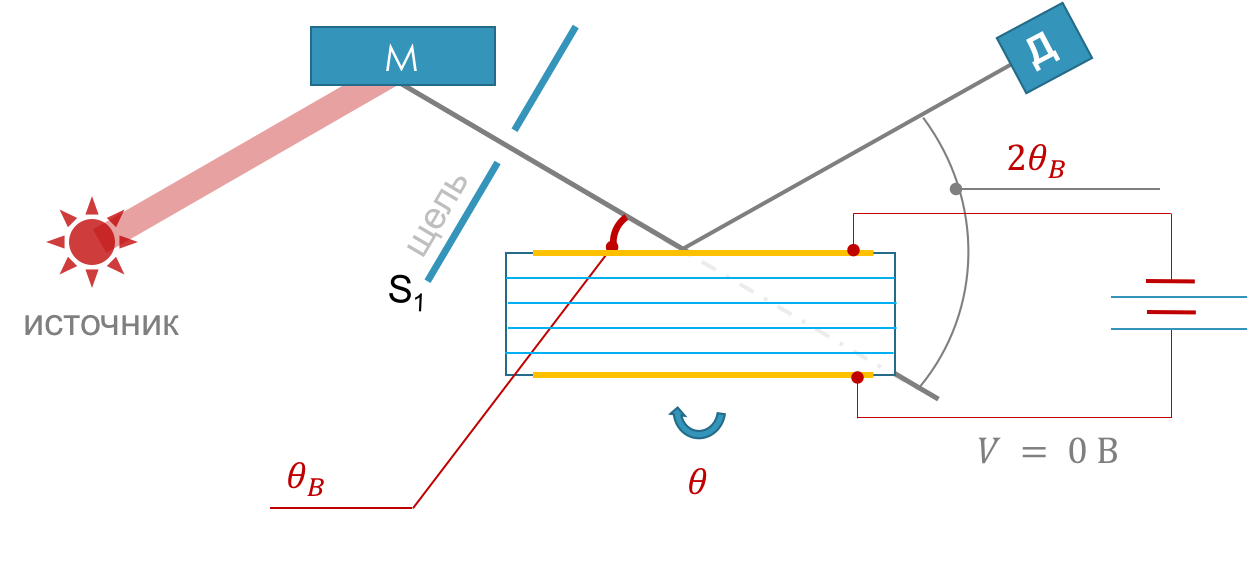
\includegraphics[width=0.33\textwidth]{images/piezo_classic_1.png}\label{ris:piezo_classic_1}}
  \hfill
  \subfloat[]{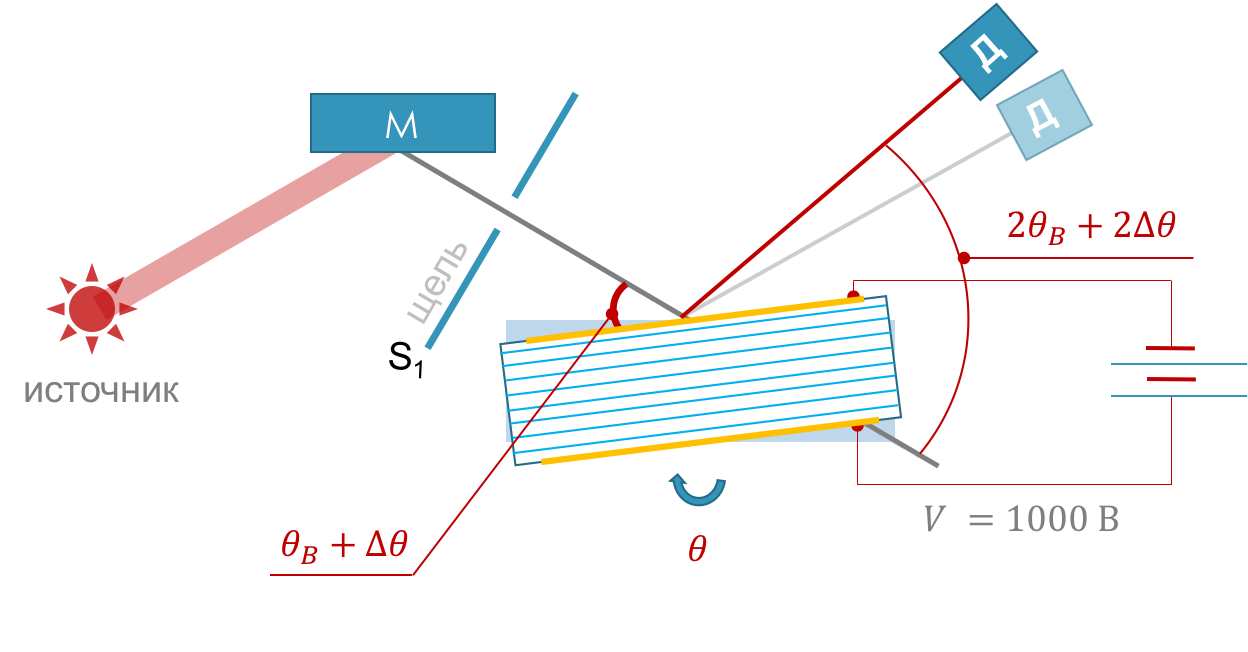
\includegraphics[width=0.33\textwidth]{images/piezo_classic_2.png}\label{ris:piezo_classic_2}}
  \hfill
  \subfloat[]{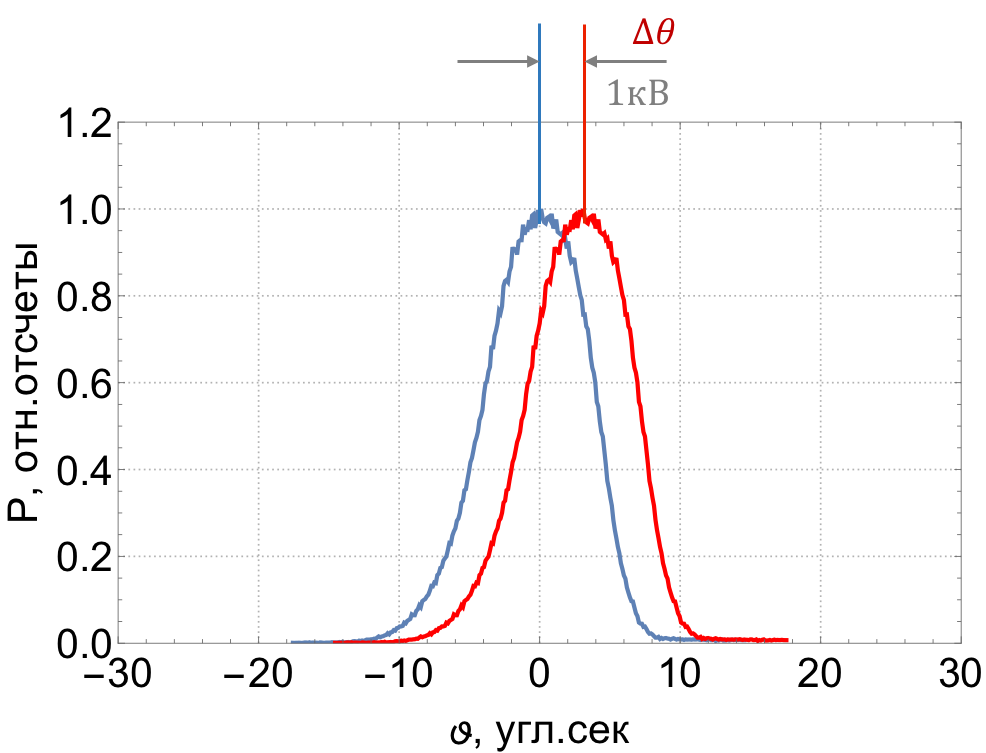
\includegraphics[width=0.2\textwidth]{images/piezo_classic_3.png}\label{ris:piezo_classic_3}}

  \caption{Схематичное представление методики измерения положения брэгговского максимума
   в отсутствии электрического поля (a), под действием электрического поля (b),
   изменение положения максимума КДО под действие электрического поля (c)}
  \label{ris:piezo_classic}
\end{figure}
  Такой метод не позволяет отследить динамику кристаллической решетки в момент приложения электрического поля,
  т.к. время за которое измеряется КДО на лабораторном источнике составляет десятки секунд.
